\documentclass[11pt]{article} 
\usepackage[english]{babel}
\usepackage[utf8]{inputenc}
\usepackage[margin=0.5in]{geometry}
\usepackage{amsmath}
\usepackage{amsthm}
\usepackage{amsfonts}
\usepackage{amssymb}
\usepackage[usenames,dvipsnames]{xcolor}
\usepackage{graphicx}
\usepackage[siunitx]{circuitikz}
\usepackage{tikz}
\usepackage[colorinlistoftodos, color=orange!50]{todonotes}
\usepackage{hyperref}
\usepackage[numbers, square]{natbib}
\usepackage{fancybox}
\usepackage{epsfig}
\usepackage{soul}
\usepackage[framemethod=tikz]{mdframed}
\usetikzlibrary{positioning, automata, backgrounds}
\usepackage[shortlabels]{enumitem}
\usepackage[version=4]{mhchem}
\usepackage{multicol}
\usepackage{forest}
\usepackage{mathtools}
\usepackage{comment}
\usepackage{enumitem}
\usepackage[utf8]{inputenc}
\usepackage[linesnumbered,ruled,vlined]{algorithm2e}
\usepackage{listings}
\usepackage{color}
\usepackage[numbers]{natbib}
\usepackage{subfiles}
\usepackage{tkz-berge}


\newtheorem{prop}{Proposition}[section]
\newtheorem{thm}{Theorem}[section]
\newtheorem{lemma}{Lemma}[section]
\newtheorem{cor}{Corollary}[prop]

\theoremstyle{definition}
\newtheorem{definition}{Definition}

\theoremstyle{definition}
\newtheorem{required}{Problem}

\theoremstyle{definition}
\newtheorem{ex}{Example}


\newcommand{\interval}[4]{\draw (#2, #1) -- (#3, #1); % Usage: \interval{height}{start}{end}{label}
\draw (#2, #1-0.11) -- (#2, #1+0.11); % draw left whisker
\draw (#3, #1-0.11) -- (#3, #1+0.11); % draw right whisker
\node[] at (#2-0.25, #1) {#4};
}

\setlength{\marginparwidth}{3.4cm}
%#########################################################

%To use symbols for footnotes
\renewcommand*{\thefootnote}{\fnsymbol{footnote}}
%To change footnotes back to numbers uncomment the following line
%\renewcommand*{\thefootnote}{\arabic{footnote}}

% Enable this command to adjust line spacing for inline math equations.
% \everymath{\displaystyle}

% _______ _____ _______ _      ______ 
%|__   __|_   _|__   __| |    |  ____|
%   | |    | |    | |  | |    | |__   
%   | |    | |    | |  | |    |  __|  
%   | |   _| |_   | |  | |____| |____ 
%   |_|  |_____|  |_|  |______|______|
%%%%%%%%%%%%%%%%%%%%%%%%%%%%%%%%%%%%%%%

\title{
\normalfont \normalsize 
\textsc{CSCI 3104 Fall 2021 \\ 
Instructor: Profs. Grochow and Waggoner} \\
[10pt] 
\rule{\linewidth}{0.5pt} \\[6pt] 
\huge Problem Set 2 \\
\rule{\linewidth}{2pt}  \\[10pt]
}
%\author{Your Name}
\date{}

\begin{document}
\definecolor {processblue}{cmyk}{0.96,0,0,0}
\definecolor{processred}{rgb}{200, 0, 0}
\definecolor{processgreen}{rgb}{0, 255, 0}
\DeclareGraphicsExtensions{.png}
\DeclareGraphicsExtensions{.gif}
\DeclareGraphicsExtensions{.jpg}

\maketitle


%%%%%%%%%%%%%%%%%%%%%%%%%
%%%%%%%%%%%%%%%%%%%%%%%%%%
%%%%%%%%%%FILL IN YOUR NAME%%%%%%%
%%%%%%%%%%AND STUDENT ID%%%%%%%%
%%%%%%%%%%%%%%%%%%%%%%%%%%
\noindent
Due Date \dotfill \textbf{September 14, 2021} \\
Name \dotfill \textbf{Michael Ghattas} \\
Student ID \dotfill \textbf{109200649} \\
Collaborators \dotfill \textbf{Me, Myself, and I}

\tableofcontents

\section{Instructions}
 \begin{itemize}
	\item The solutions \textbf{must be typed}, using proper mathematical notation. We cannot accept hand-written solutions. \href{http://ece.uprm.edu/~caceros/latex/introduction.pdf}{Here's a short intro to \LaTeX.}
	\item You should submit your work through the \textbf{class Canvas page} only. Please submit one PDF file, compiled using this \LaTeX \ template.
	\item You may not need a full page for your solutions; pagebreaks are there to help Gradescope automatically find where each problem is. Even if you do not attempt every problem, please submit this document with no fewer pages than the blank template (or Gradescope has issues with it).

	\item You are welcome and encouraged to collaborate with your classmates, as well as consult outside resources. You must \textbf{cite your sources in this document.} \textbf{Copying from any source is an Honor Code violation. Furthermore, all submissions must be in your own words and reflect your understanding of the material.} If there is any confusion about this policy, it is your responsibility to clarify before the due date. 

	\item Posting to \textbf{any} service including, but not limited to Chegg, Reddit, StackExchange, etc., for help on an assignment is a violation of the Honor Code.

	\item You \textbf{must} virtually sign the Honor Code (see Section \ref{HonorCode}). Failure to do so will result in your assignment not being graded.
\end{itemize}


\section{Honor Code (Make Sure to Virtually Sign)} \label{HonorCode}

\begin{required}
\begin{itemize}
\item My submission is in my own words and reflects my understanding of the material.
\item Any collaborations and external sources have been clearly cited in this document.
\item I have not posted to external services including, but not limited to Chegg, Reddit, StackExchange, etc.
\item I have neither copied nor provided others solutions they can copy.
\end{itemize}

%\noindent In the specified region below, clearly indicate that you have upheld the Honor Code. Then type your name. 
\end{required}

\begin{proof}[\textbf{I agree to the above, Michael Ghattas.}]
%% Typing "I agree to the above," followed by your name is sufficient.
\end{proof}



\newpage
\section{Standard 3- Dijkstra's Algorithm}

\subsection{Problem \ref{Dijkstra0}}
\begin{required} \label{Dijkstra0}
Consider the weighted graph $G(V, E, w)$ pictured below. Work through Dijkstra's algorithm on the following graph, using the source vertex $E$. 
\begin{itemize}
\item Clearly include the contents of the priority queue, as well as the distance from $E$ to each vertex at each iteration.
\item If you use a table to store the distances, clearly label the keys according to the vertex names rather than numeric indices (i.e., \texttt{dist[`B']} is more descriptive than \texttt{dist[`1']}).
\item You do \textbf{not} need to draw the graph at each iteration, though you are welcome to do so. [This may be helpful scratch work, which you do not need to include.]
\end{itemize}


\begin{center}
\begin {tikzpicture}[-latex, auto, node distance =2 cm and 3cm, semithick]
\tikzstyle{blue}=[circle ,top color =white , bottom color = processblue!20 ,draw,processblue , text=blue , minimum width =1 cm];
\tikzstyle{red}=[circle ,top color =white , bottom color = processred!20 ,draw, processred , text=blue , minimum width =1 cm];
\tikzstyle{green}=[circle ,top color =white , bottom color = processgreen!20 ,draw, processgreen , text=blue , minimum width =1 cm];

	\node[blue] (A) {$A$};
	\node[blue] (C) [below right = of A] {$C$};
	\node[blue] (B) [below right = of C] {$B$};
	\node[blue] (E) [below left = of A] {$E$};
	\node[blue] (D) [below left = of E] {$D$};
	\node[blue] (H) [below right = of D] {$H$};
	\node[blue] (F) [right = of H] {$F$};

	\path (A) edge node[above] {$3$} (C);
	\path (E) edge node[left] {$9$} (A);

	\path (C) edge node[above] {$3$} (B);
	\path (B) edge node[below] {$6$} (F);

	\path (E) edge node[above] {$15$} (C);
	\path (C) edge node[above] {$2$} (F);

	\path (H) edge node[above] {$4$} (D);

	\path (E) edge node[above] {$20$} (F);
	\path (E) edge node[right] {$9$} (H);
	\end{tikzpicture}  
\end{center}

\end{required}

\begin{proof}[Answer:]
\item \textbf{Please see the solution Graph and Table on the next page.}

\begin{center}
\begin {tikzpicture}[-latex, auto, node distance =2 cm and 3cm, semithick]
\tikzstyle{blue}=[circle ,top color =white , bottom color = processblue!20 ,draw,processblue , text=blue , minimum width =1 cm];
\tikzstyle{red}=[circle ,top color =white , bottom color = processred!20 ,draw, processred , text=blue , minimum width =1 cm];
\tikzstyle{green}=[circle ,top color =white , bottom color = processgreen!20 ,draw, processgreen , text=blue , minimum width =1 cm];

	\node[blue] (A) {$A$};
	\node[blue] (C) [below right = of A] {$C$};
	\node[blue] (B) [below right = of C] {$B$};
	\node[blue] (E) [below left = of A] {$E$};
	\node[blue] (D) [below left = of E] {$D$};
	\node[blue] (H) [below right = of D] {$H$};
	\node[blue] (F) [right = of H] {$F$};

	\path[blue] [line width=3pt] (A) edge node[above] {$3$} (C);
	\path[blue] [line width=3pt]  (E) edge node[left] {$9$} (A);

	\path[blue] [line width=3pt]  (C) edge node[above] {$3$} (B);
	\path (B) edge node[below] {$6$} (F);

	\path (E) edge node[above] {$15$} (C);
	\path[blue] [line width=3pt]  (C) edge node[above] {$2$} (F);

	\path[blue] [line width=3pt] (H) edge node[above] {$4$} (D);

	\path (E) edge node[above] {$20$} (F);
	\path[blue] [line width=3pt]  (E) edge node[right] {$9$} (H);
	\end{tikzpicture}  
\end{center}

	\begin{table}[ht]
		\caption{\textbf{Priority Queue}}
		\centering
		\begin{tabular}{|c|c|c|c|c|c|c|c|}
			\hline
			& dist[\textbf{A}] & dist[\textbf{B}] & dist[\textbf{C}] & dist[\textbf{D}] & dist[\textbf{E}] & dist[\textbf{F}] & dist[\textbf{H}] \\  [0.5ex]
			\hline 
			\textbf{1. $Source$ $Vertex$ $[E]$} & \textcolor{red}{(\textbf{9})} & (\textbf{|}) & (\textbf{15}) & (\textbf{|}) & \textcolor{red}{(\textbf{0})} & (\textbf{20}) &  \textcolor{red}{(\textbf{9})} \\ 
			\hline 
			\textbf{2. $[EH]$} & (\textbf{9}) & (\textbf{|}) & (\textbf{15}) & \textcolor{red}{(\textbf{13})} & (\textbf{0}) & (\textbf{20}) & (\textbf{9}) \\ 
			\hline
			\textbf{3. $[EH]$ $+$ $[EA]$} & (\textbf{9}) & (\textbf{|}) & \textcolor{red}{(\textbf{12})} & (\textbf{13}) & (\textbf{0}) & (\textbf{20}) & (\textbf{9}) \\  
			\hline 
			\textbf{4. $[EHD]$ $+$ $[EA]$} & (\textbf{9}) & (\textbf{|}) & (\textbf{12}) & (\textbf{13}) & (\textbf{0}) & (\textbf{20}) & (\textbf{9}) \\  
			\hline 
			\textbf{\textcolor{blue}{5. $[EHD]$ $+$ $[EAC]$}} & (\textbf{9}) & \textcolor{red}{(\textbf{15})} & (\textbf{12}) & (\textbf{13}) & (\textbf{0}) & \textcolor{red}{(\textbf{14})} & (\textbf{9}) \\
			\hline
			\textbf{6. $[EHD]$ $+$ $[EACF]$} & (\textbf{9}) & (\textbf{15}) & (\textbf{12}) & (\textbf{13}) & (\textbf{0}) & (\textbf{14}) & (\textbf{9}) \\
			\hline 
			\textbf{7. $[EHD]$ $+$ $[EACF]$ $+$ $[EACB]$} & (\textbf{9}) & (\textbf{15}) & (\textbf{12}) & (\textbf{13}) & (\textbf{0}) & (\textbf{14}) & (\textbf{9}) \\  
			\hline 
		\end{tabular} 
        \label{table:nonlin}
	\end{table}	

%Your answer here
\end{proof}





\newpage
\subsection{Problem \ref{Dijkstra2}} 
\begin{required} \label{Dijkstra2}
You have three batteries, with 4200, 2700, and 1600 mAh (milli-Amp-hours), respectively. The 2700 and 1600-mAh batteries are fully charged (containing 2700 mAh and 1600 mAh, respectively), while the 4200-mAh battery is empty, with 0 mAh. You have a battery transfer device which has a ``source'' battery position and a ``target'' battery position. When you place two batteries in the device, it instantaneously transfers as many mAh from the source battery to the target battery as possible. Thus, this device stops the transfer either when the source battery has no mAh remaining or when the destination battery is fully charged (whichever comes first).  \\

\noindent But battery transfers aren't free! The battery device is also hooked up to your phone by bluetooth, and automatically charges you a number of cents equal to however many mAh it just transfered.  \\
	
\noindent The goal in this problem is to determine whether there exists a sequence of transfers that leaves exactly 1200 mAh either in the 2700-mAh battery or the 1600-mAh battery, and if so, how little money you can spend to get this result. \\

\noindent Do the following.
\begin{enumerate}[label=(\alph*)]
\subsubsection{Problem 3\ref{Dijkstra2a}}
\item \label{Dijkstra2a} Rephrase this is as a graph problem. Give a precise definition of how to model this problem as a graph, and state the specific question about this graph that must be answered. [\textbf{Note:} While you are welcome to draw the graph, it is enough to provide 1-2 sentences clearly describing what the vertices are and when two vertices are adjacent. If the graph is weighted, clearly specify what the edge weights are.]

\begin{proof}[Answer:]

\item \textbf{The graph representing the problem would consist of multiple nodes, where each node holds the details of the current status of all the batteries.} i.e. \textbf{Node(n)}=[$(4200mAh : Status) | (2700mAh : Status) | (1600mAh : Status)$] \textbf{Further more, the edges between adjacent vertices would represent the phase transition between the batteries through charger transfer. Finally, each edge weight would be calculated based on the amount of charge transferred between two batteries. Accordingly, please see Table-2 and Table-3 for more detailed examples.}
	
	\begin{table}[ht]
		\caption{\textbf{Nodes $(Based$ $on$ $charge$ $distributions)$}}
		\centering
		\begin{tabular}{|c|c|c|c|}
			\hline
			$Vertex$  & \textbf{4200 mAh $Capacity$} & \textbf{2700 mAh $Capacity$} & \textbf{1600 mAh $Capacity$} \\  [0.5ex]
			\hline 
			V(\textbf{A}) $Source$ & \textcolor{red}{(\textbf{Empty})} & \textcolor{blue}{(\textbf{Full})} & \textcolor{blue}{(\textbf{Full})} \\ 
			\hline 
			V(\textbf{B}) & (\textbf{2700}) & \textcolor{red}{(\textbf{Empty})} & \textcolor{blue}{(\textbf{Full})} \\ 
			\hline
			V(\textbf{C}) & (\textbf{1600}) & \textcolor{blue}{(\textbf{Full})} & \textcolor{red}{(\textbf{Empty})} \\ 
			\hline 
			V(\textbf{D}) & \textcolor{blue}{(\textbf{Full})} & (\textbf{100}) & \textcolor{red}{(\textbf{Empty})} \\ 
			\hline 
			V(\textbf{E}) & \textcolor{blue}{(\textbf{Full})} & \textcolor{red}{(\textbf{Empty})} & (\textbf{100}) \\ 
			\hline
			V(\textbf{F}) & (\textbf{2700}) & (\textbf{1600}) & \textcolor{red}{(\textbf{Empty})} \\ 
			\hline
			V(\textbf{G}) & (\textbf{1600}) & (\textbf{1100}) & \textcolor{blue}{(\textbf{Full})} \\ 
			\hline
			V(\textbf{H}) & (\textbf{3200}) & (\textbf{1100}) & \textcolor{red}{(\textbf{Empty})} \\ 
			\hline
			V(\textbf{....}) & (\textbf{....}) & (\textbf{....}) & (\textbf{....}) \\ 
			\hline
			V(\textbf{etc.}) & (\textbf{etc.}) & (\textbf{etc.}) & (\textbf{etc.}) \\ 
			\hline
		\end{tabular} 
        \label{table:nonlin}
	\end{table}	
	
	\begin{table}[ht]
		\caption{\textbf{Edges $(Based$ $on$ $transfer$ $cost)$}}
		\centering
		\begin{tabular}{|c|c|c|c|c|}
			\hline
			\textcolor{blue}{$Edge$}  & \textbf{4200 mAh $Capacity$} & \textbf{2700 mAh $Capacity$} & \textbf{1600 mAh $Capacity$} & \textcolor{red}{\textbf{Weight}} \\  [0.5ex]
			\hline
			\textcolor{blue}{\textbf{AB}} & (\textbf{2700}) & (\textbf{0}) & (\textbf{1600}) &  \textcolor{red}{(\textbf{2700})} \\ 
			\hline 
			\textcolor{blue}{\textbf{AC}}  & (\textbf{1600}) & (\textbf{2700}) & (\textbf{0}) &  \textcolor{red}{(\textbf{1600})} \\ 
			\hline 
			\textcolor{blue}{\textbf{CD}}  & (\textbf{4200}) & (\textbf{100}) & (\textbf{0}) &  \textcolor{red}{(\textbf{2600})} \\ 
			\hline 
			\textcolor{blue}{\textbf{BE}}  & (\textbf{4200}) & (\textbf{0}) & (\textbf{100}) &  \textcolor{red}{(\textbf{1500})} \\ 
			\hline
			\textcolor{blue}{\textbf{BF}} & (\textbf{2700}) & (\textbf{1600}) & (\textbf{0}) & \textcolor{red}{(\textbf{1600})} \\ 
			\hline 
			\textcolor{blue}{\textbf{CG}} & (\textbf{1600}) & (\textbf{1100}) & (\textbf{1600}) & \textcolor{red}{(\textbf{1600})} \\
			\hline 
			\textcolor{blue}{\textbf{GH}}  & (\textbf{3200}) & (\textbf{1100}) & (\textbf{0}) & \textcolor{red}{(\textbf{1600})} \\ 
			\hline
			\textcolor{blue}{\textbf{....}}  & (\textbf{....}) & (\textbf{....}) & (\textbf{....}) & \textcolor{red}{(\textbf{....})} \\ 
			\hline
			\textcolor{blue}{\textbf{etc.}}  & (\textbf{etc.}) & (\textbf{etc.}) & (\textbf{etc.}) & \textcolor{red}{(\textbf{etc.})} \\ 
			\hline
		\end{tabular} 
        \label{table:nonlin}
	\end{table}	
%Your answer goes here.
\end{proof}

\newpage
\subsubsection{Problem 3\ref{Dijkstra2b}}
\item \label{Dijkstra2b} Clearly describe an algorithm to solve this problem. If you use an algorithm covered in class, it is enough to state that. If you modify an algorithm from class, clearly outline any modifications. Make sure to explicitly specify any parameters that need to be passed to the initial function call.

\begin{proof}[Answer:]
\textbf{Using Dijkstra's Algorithm, we initialization of all nodes with distance = $infinity$, while initialization the starting node to 0. We mark the distance of the starting node as permanent, and all other distances as temporarily. Then, we set the starting node as active, and perform calculations of the temporary distances of all neighboring nodes of the active node by summing up the distance based on the weights of the edges.
If the calculated distance of a node is smaller than the current one, we update the distance and set the current node as predecessor. We then set the node with the minimal temporary distance as active, and mark its distance as permanent.
We repeat steps 4 to 7 until there aren't any nodes left with a permanent distance, and which neighboring nodes still have assigned temporary distances.}

\item \textbf{function} $Dijkstra(Graph, source):$ \
\item	\hspace*{10mm} \textbf{for each} vertex $v$ in $Graph$: \
\item	\hspace*{20mm} dist[$v$] $:= infinity$ \
\item	\hspace*{20mm} previous[$v$] $:= undefined$ \
\item	\hspace*{10mm} dist[$source$] $:= 0$ \
\item	\hspace*{10mm} $Q$ $:=$ the set of all nodes in $Graph$ \
\item	\hspace*{10mm} \textbf{while} $Q$ is not $empty$:
\item	\hspace*{20mm} $u$ $:= node$ in $Q$ with $smallest$ dist[ ] \
\item	\hspace*{20mm} remove $u$ from $Q$ \
\item	\hspace*{20mm} \textbf{for each} neighbor $v$ of $u$: \
\item	\hspace*{30mm} $alt$ $:=$ dist[$u$] + $DistBetween(u, v)$ \
\item	\hspace*{30mm} \textbf{if} $alt$ $<$ dist[$v$] \
\item	\hspace*{40mm} dist[$v$] $:=$ $alt$ \
\item	\hspace*{40mm} previous[$v$] $:=$ $u$
\item	\hspace*{40mm} update(Q) \
\item \hspace*{10mm} \textbf{return} $Graph$;
%Your answer goes here
\end{proof}



\newpage
\subsubsection{Problem 3\ref{Dijkstra2c}}
\item \label{Dijkstra2c} Apply that algorithm to the question. Report and justify your answer. Here, justification includes the sequences of vertices visited and the total cost. 

\begin{proof}[Answer:]
\item \textbf{While there are sure to be multiple solutions possible through vertices with different charge combinations, using the information from part(a) and part(b) we should get the following lowest cost of operation and visited vertices:} \\

\item \textbf{V(*)[4200mAh-Capacity:$Charge$, 2700mAh-Capacity:$Charge$, 1600mAh-Capacity:$Charge$]} \\
\item \textbf{1. V(1)[4200:$0$, 2700:$2700$, 1600:$1600$]} \\
\item	\hspace*{10mm} \textbf{Edge:} $V(1) \to V(2) := weight(2700)$ \\
\item \textbf{2. V(2)[4200:$2700$, 2700:$0$, 1600:$1600$]} \\
\item	\hspace*{10mm} \textbf{Edge:} $V(2) \to V(3) := weight(1500)$ \\
\item \textbf{3. V(3)[4200:$4200$, 2700:$0$, 1600:$100$]}\\
\item	\hspace*{10mm} \textbf{Edge:} $V(3) \to V(4) := weight(2700)$ \\
\item \textbf{4. V(4)[4200:$1500$, 2700:$2700$, 1600:$100$]} \\
\item	\hspace*{10mm} \textbf{Edge:} $V(4) \to V(5) := weight(1500)$ \\
\item \textbf{5. V(5)[4200:$1500$, 2700:\textcolor{red}{$1200$}, 1600:$1600$]} \\
\item	\textbf{Cost = weight(2700) + weight(1500) + weight(2700) + weight(1500) =} \textcolor{blue}{$8400_c$} \\
%Your answer goes here
\end{proof}

\end{enumerate}
\end{required}



\newpage
\section{Standard 4- Examples Where Greedy Algorithms Fail}

\subsection{Problem \ref{GreedyFail1}}
\begin{required} \label{GreedyFail1}
Recall the \textsf{Interval Scheduling} problem, where we take as input a set of intervals $\mathcal{I}$. The goal is to find a maximum-sized set $S \subseteq \mathcal{I}$, where no two intervals in $S$ intersect. Consider the greedy algorithm where we place all of the intervals of $\mathcal{I}$ into a priority queue, ordered earliest start time to latest start time. We then construct a set $S$ by adding intervals to $S$ as we poll them from the priority queue, provided the element we polled does not intersect with any interval already in $S$. \\

\noindent Provide an example with at least $5$ intervals where this algorithm fails to yield a maximum-sized set of pairwise non-overlapping intervals. Clearly specify both the set $S$ that the algorithm constructs, as well a larger set of pairwise non-overlapping intervals. \\

\noindent You may explicitly specify the intervals by their start and end times (such as in the examples from class) or by drawing them. \textbf{If you draw them, please make it very clear whether two intervals overlap.} You are welcome to hand-draw and embed an image, provided it is legible and we do not have to rotate our screens to grade your work. Your justification should still be typed. If you would prefer to draw the intervals using \LaTeX, we have provided sample code below.
\end{required}


%Sample code to draw intervals
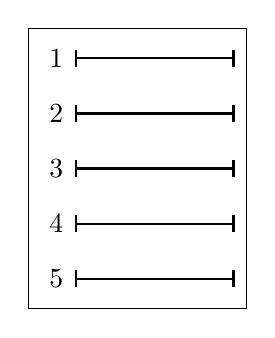
\begin{tikzpicture}[thick, framed]   
\interval{3.3}{5}{7}{1}
\interval{2.6}{5}{7}{2}
\interval{1.9}{5}{7}{3}
\interval{1.2}{5}{7}{4}
\interval{0.5}{5}{7}{5}
\end{tikzpicture}

\begin{proof}[Answer:]
\item \textbf{\\ Below is an example how the greedy algorithm fails:}
\item \hspace*{10mm} Let our set of intervals be int[$StartTime_i:EndTime_i$].
\item \textbf{Setting the order of intervals from earliest to latest start-time, left-to-right, we get our $PriorityQueue$:}
\item \hspace*{10mm} $\mathcal{I}$ = [int($1:12$) , int($2:3$) , int($4:5$) , int($6:7$) , int($8:9$), int($10:11$)]
\item \hspace*{10mm} Let our $answer$ set of intervals be $(S)$.
\item \textbf{We start to populate our stack, and we first stack} int($1:12$), thus $S$ = [int($1:12$)]
\item \hspace*{10mm} Next, due to overlap with [int($1:11$)], we realize that we are unable to add to $S$ any
\item \hspace*{10mm} of the other intervals; [int($2:3$) , int($4:5$) , int($6:7$) , int($8:9$), int($10:11$)].
\item \textbf{Thus our final solution is} $S$ $=$ [int($1:12$)]
\item \textbf{\\ However, this is clearly not the optimal solution-set where we can stack multiple intervals to our queue. The optimal solution would consider the earliest end times instead.}
\item \hspace*{10mm} Let $O$ $=$ ($Optimal$ $Solution$):
\item \hspace*{10mm} Then the optimal solution would instead be: $(O)$ $=$ [int($2:3$) , int($4:5$) , int($6:7$) , int($8:9$), int($10:11$)]
\item \textbf{Accordingly we can see how our example and provided greedy algorithm failed to provide us with the optimal solution-set for the given problem!}
%Your answer here.
\end{proof}






\newpage
\subsection{Problem \ref{GreedyFail3}}
\begin{required} \label{GreedyFail3}
Consider now the \textsf{Weighted Interval Scheduling} problem, where each interval $i$ is specified by 
\[
([\text{start}_{i}, \text{end}_{i}], \text{weight}_{i}). 
\]

\noindent Here, the weight is an assigned value that is independent of the length $\text{end}_{i} - \text{start}_{i}$. Here, you may assume $\text{weight}_{i} > 0$. We seek a set $S$ of pairwise non-overlapping intervals that maximizes $\sum_{i \in S} \text{weight}_{i}$. That is, rather than maximizing the number of intervals, we are seeking to maximize the sum of the weights. \\

\noindent Consider a greedy algorithm which works identically as in Problem \ref{GreedyFail1}. Draw an example with at least 5 appointments where this algorithm fails. Show the order in which the algorithm selects the intervals, and also show a subset with larger weight of non-overlapping intervals than the subset output by the greedy algorithm. The same comments apply here as for Problem \ref{GreedyFail1} in terms of level of explanation.
\end{required}

\begin{proof}[Answer:]
\item \textbf{\\ Below is an example how the greedy algorithm fails:}
\item \hspace*{10mm} Let our set of intervals be int[$StartTime_i:EndTime_i, Weight_i$].
\item \textbf{Setting the order of intervals from highest to lowest weight, left-to-right, we get our $PriorityQueue$:}
\item \hspace*{10mm} $\mathcal{I}$ = [int($2:12, 200$) , int($9:10, 100$) , int($7:8, 75$) , int($5:6, 50$) , int($3:4, 25$), int($1:3, 10$)]
\item \hspace*{10mm} Let our $answer$ set of intervals be $(S)$.
\item \textbf{We start to populate our stack, and we first stack} int($1:3, 10$), \textbf{then replace it with} int($2:12, 200$) \textbf{due to the higher weight and overlap. Thus initially} $S$ = [int($2:12, 200$)]
\item \hspace*{10mm} Next, due to overlap with [int($2:12, 200$)], \textbf{we realize that we are unable to add to} $S$ any of
\item \hspace*{10mm} the other intervals; [int($9:10, 100$) , int($7:8, 75$) , int($5:6, 50$) , int($3:4, 25$)], or bring back int($1:3, 10$).
\item \textbf{Thus our final solution is} $S$ $=$ [int($2:12, 200$)] $=$ $200$.
\item \textbf{\\ However, this is clearly not the optimal solution-set where we can stack to our queue multiple intervals that can add-up to a larger total weight. The optimal solution would consider the higher weight along with the earliest end times instead.}
\item \hspace*{10mm} Let $O$ $=$ ($Optimal$ $Solution$):
\item \hspace*{10mm} Then the optimal solution would instead be: $(O)$ $=$ \{[int($9:10, 100$) $+$ int($7:8, 75$) $+$ int($5:6, 50$) $+$ 
\item \hspace*{10mm} int($3:4, 25$)] $=$ [$100 + 75 + 50 + 25$ $=$ $250$]\} $>$ \{[$S$ $=$ int($2:12, 200$)] $=$ [$200$]\}, Thus [$(O)>(S)$].
\item \textbf{Accordingly we can see how our example and provided greedy algorithm failed to provide us with the optimal solution-set for the given problem!}

%Your answer here.
\end{proof}




\newpage
\section{Standard 5- Exchange Arguments}
\subsection{Problem \ref{Exchange1}}
\begin{required} \label{Exchange1}
Recall the Making Change problem, where we have an infinite supply of pennies (worth $1$ cent), nickels (worth $5$ cents), dimes (worth $10$ cents), and quarters (worth $25$ cents). We take as input an integer $n \geq 0$. The goal is to make change for $n$ using the fewest number of coins possible. \\

\noindent Prove that in an optimal solution, we use at most $2$ dimes. 
\end{required}

\begin{proof}[Answer:]
\item \textbf{We will be using the below greedy algorithm, along with the notes from the class lecture (Chapter 3 - 3.1.1). Here we take in the input (n) as per the given problem, which is the number of cents provided.} i.e. Let $n \in \mathbb{N}$  be the amount for which we wish to make change. In an optimal solution, we have at most one nickel.
\\
\item \textbf{Let $(S)$ be the multi-set of coins used to make change for $(n)$. Suppose that $(S)$ contains $k > 1$ nickels. The key idea is that we may exchange each pair of nickels for a single dime. For example, based on our above division greedy Algorithm, $k = [(2j) + r]$, where $j \in \mathbb{N}$ and $r \in{[0,1]}$. When $k > 1$, $j \geq 1$. We exchange $(2j)$ nickels for $(j)$ dimes, and so on, to obtain a new optimal solution set $|$$S'$$|$, where $|$$S'$$|$ $=$ [($|$$S$$|$ $-$ $j$) $<$ $|$$S$$|$].} \\

\item $Algorithm$ $pseudocode:$ \\

\item \textbf{function} $CoinSort(n):$										
	\item	\hspace*{10mm} Count = [Quarters, Dimes, Nickels, Pennies]
	\item	\hspace*{10mm} Quarters = 0
	\item	\hspace*{10mm} Dimes = 0
	\item	\hspace*{10mm} Nickels = 0
	\item	\hspace*{10mm} Pennies = 0

	\item	\hspace*{10mm} \textbf{while} $(n$ $!=$ $0):$
	
		\item	\hspace*{20mm} \textbf{if} $(n \% 25):$
			\item	\hspace*{30mm} $n = (n-25)$
			\item	\hspace*{30mm} Quarters++
			
		\item	\hspace*{20mm} \textbf{else if} $(n \% 10):$
			\item	\hspace*{30mm} $n = (n-10)$
			\item	\hspace*{30mm} Dimes++

		\item	\hspace*{20mm} \textbf{else if} $(n \% 5):$
			\item	\hspace*{30mm} $n = (n-5)$
			\item	\hspace*{30mm} Nickels++
			
		\item	\hspace*{20mm} \textbf{else}
			\item	\hspace*{30mm} $n = (n-1)$
			\item	\hspace*{30mm} Pennies++
			
\item	\hspace*{10mm} \textbf{return}$(Count);$
%Your proof here
\end{proof}



\newpage
\subsection{Problem \ref{Exchange2}}
\begin{required} \label{Exchange2}
Consider the \textsf{Interval Projection} problem, which is defined as follows.
\begin{itemize}
\item \textsf{Instance:} Let $\mathcal{I}$ be a set of intervals on the real line.
\item \textsf{Solution:} A minimum sized set $S$ of points on the real line, such that (i) for every interval $[s, f] \in \mathcal{I}$, there exists a point $x \in S$ where $x$ is in the interval $[s, f]$. We call $S$ a \textit{projection set}.
\end{itemize}

\noindent Do the following. 
\begin{enumerate}[label=(\alph*)]
\subsubsection{Problem 7\ref{6a}}
\item \label{6a} Find a minimum sized projection set $S$ for the following set of intervals:
\begin{align*}
\mathcal{I} = \{ [0, 1], [0.5, 1], [1, 1.5], [1.4, 2], [1.6, 2.3] \}.
\end{align*}


\begin{proof}[Answer:]
\item \textbf{Let $\mathcal{I}$ be made of the intervals:} \\
$A$ = [0,1] \\
$B$ = [0.5,1] \\
$C$ = [1,1.5] \\
$D$ = [1.4,2] \\
$E$ = [1.6,2.3] \\

\item \textbf{Let $\mathcal{K}$ = [Set of overlapping intervals]}
\item \textbf{$\mathcal{K}$ = \{[0.5,1] , [1.4,1.5] , [1.6,2]\}} \\
\item \textbf{Let $\mathcal{K}$ be made of the intervals:} \\
$\alpha$ = [0.5,1] \\
$\beta$ = [1.4,1.5] \\
$\gamma$ = [1.6,2] \\

\item \textbf{We can note that:} \\
The interval $\alpha$ has the point \textbf{1} $\in$ ($A$, $B$ \& $C$) \\
The interval $\gamma$ has the point \textbf{2} $\in$ ($D$ \& $E$) \\

\item \textbf{If $\mathcal{S}$ represents the projection set, then we can clearly note that the set of points \{1,2\} represents the intervals $\in$ $\mathcal{I}$. Thus:} \\
\item \textbf{$\mathcal{S}$ = \{1, 2\}}
\item \textbf{$|$$\mathcal{S}$$|$ $=$ (2)}
%Your Answer Here
\end{proof}

\newpage
\subsubsection{Problem 7\ref{6b}}
\item \label{6b} Fix a set of intervals $\mathcal{I}$, and let $S$ be a projection set. Prove that there exists a projection set $S^{\prime}$ such that (i) $|S^{\prime}| = |S|$, and (ii) where every point $x \in S^{\prime}$ is the right end-point of some interval $[s, f] \in \mathcal{I}$. 

\begin{proof}[Answer:]
\item \textbf{Let $\mathcal{I}$ is made of a set of intervals, where each $interval_i$ is made of a set of points encapsulated by a start-point ($s_i$) and an end-point ($f_i$).}
\item \textbf{We assume each $interval_i$ is made of $[s_i,...,f_i]$$\in \mathbb{R}$, where $s_i \leq x_i \leq f_i$.}
\item \textbf{We assume $\forall$ $interval_i$ $\in$ $\mathcal{I}$ ($f_1 \leq f_i \leq f_{i+1} \leq f_n$).}
\item \textbf{We assume $x_i$ $\in$ $\forall$ $interval_i$ $\in$ $\mathcal{I}$, then $x_i$ $\in$ $\mathcal{S}$.}

\item \textbf{Let $\delta$ = [Interval with least end-point]. i.e. $f_1$ $\in$ $\delta$.} 
\item \textbf{Let $\delta$($x_i$) = $\epsilon$ = ($f_1$), where we have intervals intersecting at $\epsilon$, and $\epsilon$ = $f_{\delta}$ = $f_1$.}
\item \textbf{Then $\epsilon \in \mathcal{S}$, and $\epsilon \in \mathcal{S'}$.}
\item \textbf{Repeating this process $(n)$ times will give us $\mathcal{S}$, where $|$$\mathcal{S}$$|$ $=$ $|$$\mathcal{S'}$$|$.}
%Your proof here
\end{proof}

\end{enumerate}
\end{required}
 
\end{document} % NOTHING AFTER THIS LINE IS PART OF THE DOCUMENT



